% !TeX spellcheck = en_GB
%__________________________________________________
% Basic Template for the use in the UCLA Brain Tumor Imaging Laboratory
%	purpose: any
%__________________________________________________

%Type of document
\PassOptionsToPackage{svgnames}{xcolor}
\documentclass[12pt, letterpaper]{article}

% encoding for the document
\usepackage[utf8]{inputenc}

% include graphics
\usepackage{graphicx}

% foot note
\usepackage{fancyhdr}
\usepackage{lastpage}

% margin
\usepackage[doublespacing]{setspace}
\usepackage[margin=1.4cm]{geometry}

% Times font
\usepackage{mathptmx}

% include logos on .eps format
\usepackage{epstopdf}
% for table formating
\usepackage{array}
% for symbols
\usepackage{latexsym}
% for boxes
\usepackage{tcolorbox}
\tcbuselibrary{skins,breakable}
\usepackage{multicol}

% use tables
\usepackage[table]{colortbl}
\usepackage{booktabs}
\usepackage{hhline}

% use symbols
\usepackage{amssymb}
\usepackage{amsmath}

%%-----------Costume---------
\setlength{\parindent}{0in}

%%-----------Background------
\usepackage{eso-pic}
\newcommand\BackgroundPic{%
\put(0,0){%
\parbox[b][\paperheight]{\paperwidth}{%
\centering
\includegraphics[width=\paperwidth,height=\paperheight]{background_noLogo.png}%
}}}

%%-----------Box------
\tcbset{
colback=white,
colframe=black!15!white,
coltitle=black,
nobeforeafter,
sharp corners=uphill,
width=(\linewidth)}

\pagestyle{empty}

\begin{document}

\AddToShipoutPicture{\BackgroundPic}

%---------- Footnote---------------
\pagestyle{fancy}
\fancyhf{}
\renewcommand{\headrulewidth}{0pt}

% \lfoot{
% \vspace*{-64pt}
% \footnotesize\textit{UCLA Brain Tumor Imaging Laboratory \\
% Center for Computer Vision and Imaging Biomarkers \\
% Department of Radiology, David Geffen School of Medicine \\
% 924 Westwood Blvd., Suite 615 Los Angeles, CA 90024
% }}

\rfoot{
\vspace*{-48pt}
\footnotesize\textit{Page \thepage \hspace{1pt} of \pageref{LastPage}\\
Report Date: \today}}

%---------- TITLE ---------------
\textbf{{\Large CEST Phantom \\ Quality Assurance Report}}
\vspace*{16pt}

%---------- Scanner information ---------------
\begin{tcolorbox}
[title = \textbf{Scanner Information},
width=7cm,
height=5cm,
left skip=0cm]
\footnotesize{\input{ScanInformation.txt}}
\end{tcolorbox}
\begin{tcolorbox}
[title = \textbf{Physical Phantom Structure},
width=12cm,
height=5cm,
left skip=0.5cm]
\includegraphics[width=3.3cm]{rack_3d.png}
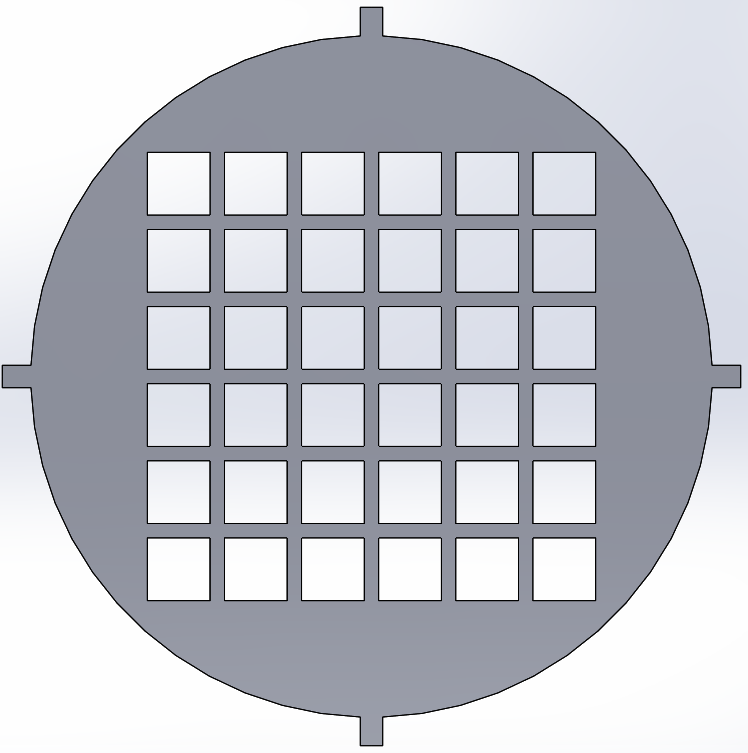
\includegraphics[width=3.3cm]{Grid_Platform.png}
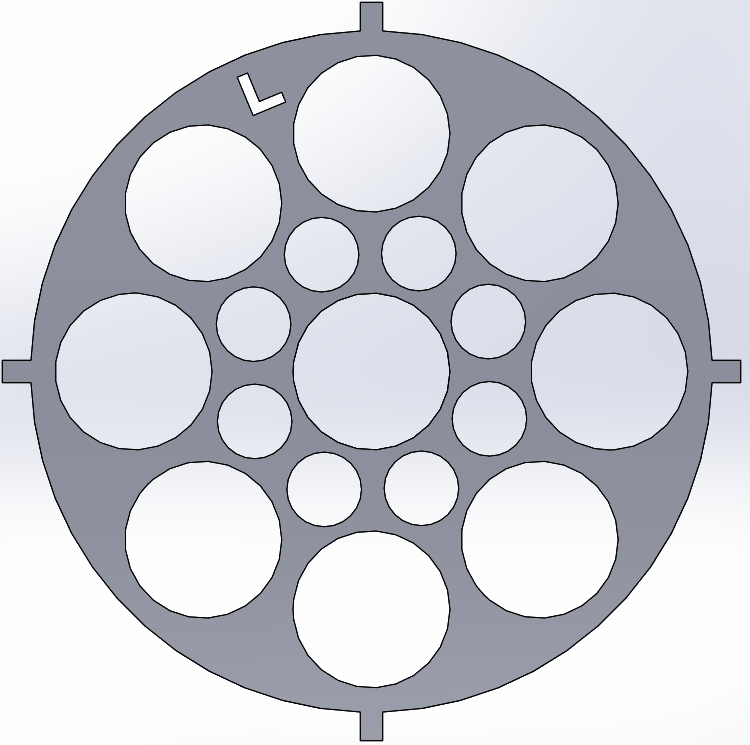
\includegraphics[width=3.3cm]{Vial_Platform.png}
\end{tcolorbox}

\vspace*{16pt}
%---------- Sequence information anatomic ---------------
\begin{tcolorbox}
[title = \textbf{Sequence Information - \textit{Anatomic}},
width=11.5cm,
height=8cm,
left skip=0cm]
\begin{multicols}{2}

\footnotesize{\input{T1w.txt}}

\columnbreak

\footnotesize{\input{T2w.txt}}

\end{multicols}
\end{tcolorbox}
\begin{tcolorbox}
[title = \textbf{CEST Saturation Parameters},
width=7.5cm,
height=8cm,
left skip=0.5cm]
\footnotesize{
\textbf{Pulse Shape}: Gaussian \\
\textbf{Pulse Length}: 100 ms \\
\textbf{Pulse Flip Angle}: 3090 degree \\
\textbf{Pulse Interval}: 5 ms \\
\textbf{Pulse Number}: 3 \\
\textbf{Offset Frequencies}: 0, $\pm$0.25, $\pm$0.5, $\pm$0.75. $\pm$1, $\pm$1.25, $\pm$1.5, $\pm$1.75, $\pm$2, $\pm$2.2, $\pm$2.4, $\pm$2.6, $\pm$2.8, $\pm$3, $\pm$3.2, $\pm$3.4, $\pm$3.6, $\pm$3.8, $\pm$4, $\pm$4.5, $\pm$5, $\pm$7, $\pm$10 ppm
}
\end{tcolorbox}

\vspace*{16pt}
%---------- Registration checking ---------------
\begin{tcolorbox}
[title = \textbf{Registration to Template - $T_2w$},
width=19.1cm,
left skip=0cm]
\begin{multicols}{2}
\footnotesize{Middle slices of coronal view, saggital view, and axial view.}

\smallskip
\includegraphics[height=3cm]{imgReg_mid.png} 

\columnbreak
\footnotesize{Slices across the three colored platforms.}

\smallskip
\includegraphics[height=3cm]{imgReg_sli.png}
\end{multicols}

\vspace*{-16pt}
\footnotesize{Note: Here we demonstrate composite RGB images showing template $T_2w$ images and acquired $T_2w$ images overlaid in different color bands. Gray regions in the composite image show where the two images have the same intensities. Magenta and green regions show where the intensities are different.}
\end{tcolorbox}

\pagebreak
\textbf{{\Large CEST Phantom \\ Quality Assurance Report}}

\vspace*{16pt}
%---------- Sequence information mappings ---------------
\begin{tcolorbox}
[title = \textbf{Sequence Information - \textit{Mappings}},
width=19.1cm,
left skip=0cm]
\begin{multicols}{3}

\footnotesize{\input{T1map.txt}}

\columnbreak

\footnotesize{\input{T2map.txt}}

\columnbreak

\footnotesize{\input{CEST.txt}}

\end{multicols}
\end{tcolorbox}

\vspace*{12pt}
%---------- Summary results ---------------
\begin{tcolorbox}
[title = \textbf{Summary of MRI Measurements (mean $\pm$ SD)},
width=19.1cm,
left skip=0cm]
\renewcommand{\arraystretch}{0.73}
\footnotesize{                 
\input{MeasurementTable.txt}                  
}
\vspace*{-8pt}
\singlespacing{
\footnotesize{Note: Colored cell indicates deviation from ground truth values. Red means higher and blue means lower than the standard values. Cell with colored text indicates that the deviation is outside the 99\% confidence interval of the standard value.}}
\end{tcolorbox}

\pagebreak
\textbf{{\Large CEST Phantom \\ Quality Assurance Report}}

\vspace*{16pt}
%---------- relaxometry and CEST results ---------------
\onehalfspacing{
\begin{tcolorbox}
[title = \textbf{Longitudinal Relaxation\\ Rate Estimation}, % \\ - $T_1$ $(ms)$
width=6cm,
height=10.5cm,
left skip=0cm]
\centering
\includegraphics[width=5cm]{T1plot.png}

\bigskip
\includegraphics[width=5cm]{T1map.png}
\end{tcolorbox}
\begin{tcolorbox}
[title = \textbf{Transverse Relaxation\\ Rate Estimation}, % \\ - $T_2$ $(ms)$
width=6.5cm,
height=10.5cm,
left skip=0.5cm]
\centering
\includegraphics[width=5cm]{T2plot.png}

\bigskip
\includegraphics[width=5cm]{T2map.png}
\end{tcolorbox}
\begin{tcolorbox}
[title =\textbf{CEST Measurement\\ - $MTR_{asym}$ $at$ $3.0ppm$ $(\%)$},
width=6.5cm,
height=10.5cm,
left skip=0.5cm]
\centering
\includegraphics[width=5cm]{MTRasymplot.png}

\bigskip
\includegraphics[width=5cm]{MTRasymmap.png}
\end{tcolorbox}
}

\vspace*{16pt}
%---------- Quality Assurance ---------------
\begin{tcolorbox}
[title = \textbf{Report Summary},
width=19.1cm,
left skip=0cm]
\small{
\input{QA.txt}   
}
\end{tcolorbox}

%---------- end CONTENT ---------------

\end{document}
}
